\question[10] Completa la Tabla \ref{tab:perimetro_lado} que muestra cómo cambia el perímetro de un cuadro
al variar la longitud de su lado.

\begin{table}[H]
    \centering
    \caption{Tabla que relaciona la medida de los lados en un cuadrado con respecto al perímetro.}
    \label{tab:perimetro_lado}
    \begin{tabular}{c|c|c|c|c}
        Lado (cm)      & 0.5 & 1 & 2 & $\dfrac{5}{2}$ \\
        \hline
        Perímetro (cm) &     &   & 8 &                \\
        \bottomrule
    \end{tabular}
\end{table}

\begin{parts}
    \part ¿Cuál es el valor de la constante de proporcionalidad?
    \part ¿Cuánto mide el lado de un cuadrado cuyo perímetro es cero?
    \part ¿Cómo es el perímetro de un cuadrado que por lado mide 4 cm con respecto a otro cuadrado cuya longitud por lado es de 2 cm?
    \part ¿Cómo se relaciona el perímetro de un cuadrado que por lado mide 4 cm con otro que mide 12 cm por lado?
    \part ¿Cómo es la relación entre el perímetro de un cuadrado y la medida de uno de sus lados?
    \part Escribe un procedimiento para obtener el perímetro de un cuadrado si conocen cuánto mide por lado.
    \part ¿Cuánto mide el lado de un cuadrado cuyo perímetro es de 1 cm?
    \part ¿Cuál de las gráficas representa la relación entre la longitud por lado y el perímetro de un cuadrado?
    \begin{figure}[H]
        \centering
        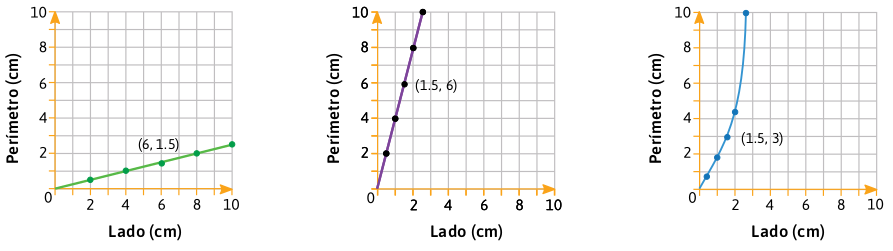
\includegraphics[width=0.45\textwidth]{../images/q70a}
        \caption{}
        \label{fig:q70a}
    \end{figure}
    \part La gráfica que representa cómo cambia el perímetro con respecto a la longitud de su lado es creciente. ¿Por qué creen que recibe ese nombre?
\end{parts}